\documentclass[11pt]{article}

\usepackage[margin=1in]{geometry}
\usepackage[T1]{fontenc}
\usepackage{lmodern}
\usepackage{microtype}
\usepackage{amsmath,amssymb}
\usepackage{booktabs}
\usepackage{xcolor}
\usepackage{tikz}
\usepackage[numbers,sort&compress]{natbib}
\usepackage[hidelinks]{hyperref}

\definecolor{ink}{HTML}{1E2A4A}
\definecolor{lumina}{HTML}{C9842A}

\title{\textcolor{ink}{A Local Lamp for Scientific Manuscripts}\\[0.35em]
\large A sample note shipped with Lumina}
\author{The Lumina Sample Project}
\date{}

\begin{document}
\maketitle

\begin{abstract}
This note is the sample project that opens with Lumina.
It is a small multi-file manuscript: prose split across section files, a table, a displayed equation, a TikZ diagram, and a bibliography of works that exist in the public record.
One bibliography entry is synthetic and labeled as such, so the citation checker has an unmatched row to report.
Typesetting does not depend on a hosted editor.
\end{abstract}

\section{The manuscript is the source}
\label{sec:intro}

Line breaking is an old problem with a precise solution.
Knuth and Plass showed that a paragraph can be set by optimizing the whole paragraph rather than filling each line in turn \cite{knuth1981breaking}.
A scientific manuscript is the same kind of object: a source file, a bibliography, and a compile you can run again.
Leslie Lamport's account of \LaTeX{} still describes that workflow \cite{lamport1994latex}.

What travels poorly is everything a hosted editor keeps beside the source.
Inline comments, collaborator permissions, and a live library connection are not the paper.
The FAIR principles ask that scholarly data be findable, accessible, interoperable, and reusable \cite{wilkinson2016fair}.
A folder of \LaTeX{} is a modest form of that claim.
If you still have the sources, you can typeset the work on a machine you control.

\section{Compile logs and citation hygiene}
\label{sec:practice}

A compile log is a sharper critic than a fluent paragraph.
When a control sequence is undefined, the engine names the file and the line.
An assistant that cannot see that log will rewrite the wrong passage and sound confident about it.
The score below is the token overlap Lumina uses when a bibliography entry has no DOI and must be compared with a public record.
$W(t)$ is the set of significant words in the bibliography title, and $W(c)$ is the same for a candidate record.

\begin{equation}
  \mathrm{score}(t, c) = \frac{2 \lvert W(t) \cap W(c) \rvert}{\lvert W(t) \rvert + \lvert W(c) \rvert}
  \label{eq:dice}
\end{equation}

A high score is not, by itself, a verification.
The checker also looks at year and the first author's family name, and it says ``unverified'' when the agreement is only partial.
Figure~\ref{fig:desk} is drawn with TikZ so this sample has no binary asset to misplace.

\begin{figure}[ht]
  \centering
  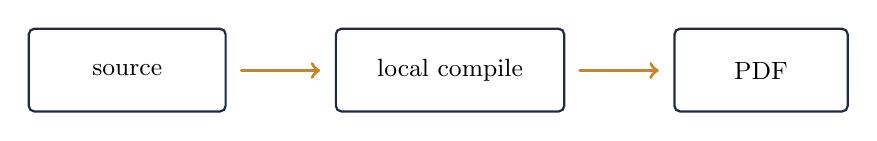
\begin{tikzpicture}[x=1cm,y=1cm,line cap=round]
    \draw[ink, thick, rounded corners=2pt] (0,0) rectangle (2.5,1.05);
    \node at (1.25,0.52) {\small source};
    \draw[lumina, very thick, ->] (2.7,0.52) -- (3.7,0.52);
    \draw[ink, thick, rounded corners=2pt] (3.9,0) rectangle (6.8,1.05);
    \node at (5.35,0.52) {\small local compile};
    \draw[lumina, very thick, ->] (7.0,0.52) -- (8.0,0.52);
    \draw[ink, thick, rounded corners=2pt] (8.2,0) rectangle (10.4,1.05);
    \node at (9.3,0.52) {\small PDF};
  \end{tikzpicture}
  \caption{The manuscript stays in a project folder. Compilation is a local step.}
  \label{fig:desk}
\end{figure}

\begin{table}[ht]
  \centering
  \begin{tabular}{lp{7.2cm}}
    \toprule
    State & How to read it \\
    \midrule
    Verified & A Crossref, OpenAlex, or arXiv record agrees with the entry. \\
    Mismatch & An identifier resolved, but the title does not agree. \\
    Unverified & No confident public match. This is not a claim that the work is fake. \\
    Missing & A citation key appears in the source and in no bibliography file. \\
    Could not check & The lookup itself failed. Try again when the network is reachable. \\
    \bottomrule
  \end{tabular}
  \caption{Statuses in a Lumina citation report.}
  \label{tab:status}
\end{table}

Fluent drafting makes invented references easier to miss.
Attention-based models made that fluency ordinary \cite{vaswani2017attention}.
Fluency is not a bibliographic record.
The key \texttt{luminaDemoUnverifiable2099} points at a synthetic entry in \texttt{refs.bib}.
It is not a real work, and the checker should refuse to mark it verified.

\section{What to keep}
\label{sec:closing}

Keep the source under your own control, compile it with a real engine, and treat a citation as verified only after a public index agrees.
Lumina is one workspace for that habit.
It is not the only editor that can open a \LaTeX{} project, and it does not need to be.
The part that matters is that the files, the log, and the decision to accept an edit stay with you.


\bibliographystyle{plainnat}
\bibliography{refs}

\end{document}
